\documentclass[11pt]{article}
\usepackage[a4paper,margin=2.2cm]{geometry}
\usepackage[T1]{fontenc}
\usepackage{lmodern}
\usepackage{microtype}
\usepackage{amsmath}
\usepackage{booktabs}
\usepackage{graphicx}
\usepackage[numbers,sort&compress]{natbib}
\usepackage[hidelinks]{hyperref}
\usepackage{xurl}
\usepackage[section]{placeins}
\usepackage{caption}
\captionsetup{skip=6pt,font=small}
% Generated tables use table* (two-column venues); in this one-column report they float like table
\makeatletter
\renewenvironment{table*}[1][]{\@float{table}[!htbp]}{\end@float}
\makeatother

% Tables and figures are generated from the evaluation results; they are never edited by hand
\graphicspath{{../../results/final_eval/figures/}}
\newcommand{\tbl}[1]{\input{../../results/final_eval/paper/#1.tex}}

\title{How Far Do Small Open Language Models Go Zero-Shot?\\[2pt]
\large Refusal-Aware Evaluation of Sexism Detection and Categorisation on CMSB, EDOS and EXIST~2025}
\author{Pawan Sapkota Sharma}
\date{October 2026}

\begin{document}
\maketitle

\begin{center}
\small\textit{Content note: this report concerns sexist language. No examples of such language are reproduced.}
\end{center}

\begin{abstract}
Detecting online sexism, and distinguishing its forms, usually relies on large expert-annotated training sets. We examine how far small open-weight instruction-tuned language models (at most 8B parameters) go as zero-shot classifiers, and how they should be scored when they do not answer in the required format. Fifteen models are evaluated on seven tasks from three benchmarks: CMSB, EDOS Tasks A--C, and the English portion of EXIST~2025 Tasks 1.1--1.3. Labels are read from the next-token probabilities of the valid answer tokens rather than from generated text. A label whose valid answers receive less than half of the probability mass is treated as a non-answer and scored as an error. All decision rules and statistical tests were fixed before test labels were accessed. On binary detection the best models reach macro-F1 0.821 on CMSB and 0.712 on EDOS~A, and several 3--4B models are not significantly different from the best model. Fine-grained categorisation remains difficult: 0.508 on the four EDOS categories and 0.256 on the eleven EDOS vectors, below supervised systems on the same test set. Three models leave 81--99\% of the 11-way EDOS questions unanswered, so the treatment of non-answers materially changes their scores. Most models predict the sexist class more often than annotators do. EXIST results await the organisers' official evaluation.
\end{abstract}

\section{Introduction}\label{sec:intro}
Automatic sexism detection supports content moderation and the study of online abuse. Its most useful form goes beyond a binary decision to the type of sexism expressed, such as threats, derogation, stereotyping or condescension. Benchmarks for this task \citep{samory2021callme,kirk2023semeval,plaza2025exist} come with thousands of expert-annotated examples, and the strongest published systems are supervised models trained on them \citep{kirk2023semeval}. Building such training data for a new platform, language or taxonomy is costly.

Instruction-tuned language models offer a different route. A model can be given a written definition of a category and asked whether a post belongs to it, with no task-specific training. Small open-weight models make this practical in settings where cost, latency or data protection rule out large hosted models, because they run locally on a single GPU. Prior work shows that zero-shot prompting can be competitive for coarse abusive-language detection but trails supervised models on finer distinctions \citep{plazadelarco2023respectful,ziems2024css,riahisamani2025rlhf}. It also shows that results depend on how categories are defined in the prompt \citep{reuver2025tell}.

Evaluating such models raises a methodological problem that is easy to overlook. A model asked to answer with a single letter or with \emph{Yes}/\emph{No} may instead begin a free-text explanation, or decline to engage with offensive content \citep{rottger2024xstest}. If the most probable valid answer is read off regardless, these cases silently become predictions. If they are discarded, models are compared on different posts.

We therefore study three questions. (i) How far does zero-shot prompting of small open models go, from binary detection to 11-way categorisation? (ii) Where does it fail? (iii) How much does the treatment of non-answers change the conclusions? Our contributions are:
\begin{itemize}
  \item a test-set evaluation of 15 open instruct models ($\leq$8B parameters) on seven tasks from three benchmarks, with bootstrap confidence intervals and paired significance tests against the best model of each task;
  \item a non-answer-aware scoring procedure for log-probability classifiers, which records non-answers per post and label and reports how results change under alternative non-answer thresholds declared in advance;
  \item an analysis of non-answers, class confusions, over-prediction, calibration and inter-model agreement, which locates where zero-shot categorisation breaks down.
\end{itemize}

\section{Related work}\label{sec:related}
\paragraph{Sexism benchmarks.} CMSB \citep{samory2021callme} grounds a binary sexism label in psychological scales and adds adversarial modifications of sexist posts. EDOS, SemEval-2023 Task~10 \citep{kirk2023semeval}, introduced a hierarchical taxonomy: binary detection (Task~A), four categories (Task~B) and eleven fine-grained vectors (Task~C). Its leaderboard was led by supervised and prompt-tuned ensembles. EXIST~2025 \citep{plaza2025exist} covers sexism identification, source intention and multi-label categorisation in English and Spanish. It keeps every annotator's label and evaluates against both majority (hard) and distributional (soft) gold labels.

\paragraph{Zero-shot language models for abusive language.} \citet{plazadelarco2023respectful} show that zero-shot prompting can detect hate speech but is sensitive to model and prompt choice. In a broad benchmark of computational-social-science labelling tasks, \citet{ziems2024css} find that zero-shot models are useful but generally do not surpass fine-tuned classifiers. For sexism specifically, \citet{riahisamani2025rlhf} report zero-shot results for 7--8B models on EDOS far below supervised systems. \citet{reuver2025tell} show that the definition supplied in the prompt changes zero-shot detection, which motivates our use of each dataset's own definitions.

\paragraph{Reading labels from token probabilities.} Scoring label words by their language-model probability goes back to verbaliser-based classification \citep{schick2021exploiting}. Probability is spread over surface variants of the same answer \citep{holtzman2021surface}, which is why we sum over answer-token variants. Label-token probabilities are also biased towards particular answers, so they benefit from calibration \citep{zhao2021calibrate}. For instruction-tuned models, the first-token answer can disagree with the answer the model would write out \citep{wang2024myanswer}, and results vary with prompt formatting \citep{sclar2024quantifying}. We return to both points in Section~\ref{sec:limits}.

\section{Data}\label{sec:data}
\paragraph{Gold labels.} Models are scored against \emph{gold labels}: the reference labels assigned to each post by the datasets' annotators. EXIST provides two forms. The \emph{hard} gold keeps the class chosen by more than three of six annotators for Task~1.1, by more than two for Task~1.2, and every class chosen by more than one annotator for the multi-label Task~1.3; tweets without such a majority are excluded. The \emph{soft} gold gives the share of annotators choosing each class \citep{plaza2025exist}.

\paragraph{Splits.} Table~\ref{tab:tasks} lists the tasks and splits. EDOS and EXIST use their official splits. CMSB has no official split, so we use a fixed 70/10/20 split, grouped so that each original post, its adversarial modifications and duplicate texts fall in the same part. The training and development splits are reserved for training supervised models. The zero-shot models use no labelled data of any split, and all their decision rules are fixed a priori (Section~\ref{sec:protocol}).

\begin{table}[t]
\centering\footnotesize
\caption{Tasks and splits. Counts are posts; CMSB counts are for the annotated subset used here (in parentheses: all posts in the split). All tasks of a dataset share its splits. EDOS B/C are scored on the 970 sexist test posts. EXIST test labels are withheld by the organisers (Section~\ref{sec:exist}).}\label{tab:tasks}
\begin{tabular}{lllrrr}
\toprule
Dataset & Task & Type, classes & Train & Dev & Test \\
\midrule
CMSB \citep{samory2021callme} & binary & binary & 3{,}954 (9{,}543) & 566 (1{,}363) & 1{,}126 (2{,}725) \\
EDOS \citep{kirk2023semeval} & A & binary & 14{,}000 & 2{,}000 & 4{,}000 \\
 & B & multi-class, 4 categories & & & 970 \\
 & C & multi-class, 11 vectors & & & 970 \\
EXIST 2025, English \citep{plaza2025exist} & 1.1 & binary & 3{,}260 & 489 & 978 \\
 & 1.2 & multi-class, 4 intentions & & & 978 \\
 & 1.3 & multi-label, 5 categories & & & 978 \\
\bottomrule
\end{tabular}
\end{table}

\paragraph{CMSB.} We use the posts that carry crowd annotations. The remaining posts come from a source that is non-sexist by construction and has no annotations, so including them would let a model succeed by recognising the source. The test split has 1{,}126 annotated posts, 361 of them sexist. After text normalisation, 3 of these posts have the same text as a training or development post. We report results with and without them, for later comparison with supervised models.

\paragraph{EDOS.} The official test split has 4{,}000 posts, 970 of them sexist (24.25\%). Following the shared task, Tasks~B and~C are evaluated on the sexist posts only: ``Only sexist instances are included in Task B and C'' \citep{kirk2023semeval}. The gold Task~B labels are derogation (454), animosity (333), prejudiced discussions (94) and threats (89). The eleven Task~C vectors range from 205 posts (2.1, descriptive attacks) to 14 (3.4, condescending explanations).

\paragraph{EXIST 2025.} We use the 978 English test tweets. The organisers released the test tweets without their gold labels, as is usual in shared tasks, so systems cannot be tuned on the test answers. Test scores are obtained from the organisers' evaluation service (Section~\ref{sec:exist}).

\paragraph{Preprocessing.} All models receive the same normalised text. HTML entities are unescaped, the text is NFC-normalised, user mentions and URLs are replaced by \texttt{[USER]} and \texttt{[URL]}, and whitespace is collapsed. No lowercasing is applied.

\section{Method}\label{sec:method}
\paragraph{Models.} We evaluate 15 open-weight instruction-tuned models from 15 families, each with at most 8B total parameters according to its model card. They range from EXAONE-4.0-1.2B to Llama-3.1-8B (Appendix Table~\ref{tab:models}). Every model is pinned to a fixed repository revision.

\paragraph{Prompts.} Each task uses a single fixed zero-shot prompt for all models (Appendix~\ref{app:prompts}). A system message states that the model is an expert annotator labelling social media posts (tweets, for EXIST) for sexism. Category definitions are adapted and abridged from each dataset's own taxonomy: \citet{samory2021callme} for CMSB, \citet{kirk2023semeval} for EDOS, and the EXIST~2025 annotation guidelines. The post is enclosed in triple quotation marks.

Binary and multi-label tasks ask one question per label, giving the label's definition and requesting \emph{Yes} or \emph{No}. EXIST~1.3 therefore asks five independent questions per tweet, and a tweet for which no category is affirmed is labelled not sexist. Multi-class tasks list all classes as lettered options with their definitions, in the fixed order of the official label set, and ask for one letter. Prompts are formatted with each model's chat template and generation prompt, with reasoning (``thinking'') modes disabled and no prefilled reply.

\paragraph{Log-probability scoring.} We read the next-token distribution $p(\cdot)$ at the first reply position. For a Yes/No question,
\begin{equation*}
P(\text{Yes}) = \sum_{t \in V_{\text{Yes}}} p(t), \qquad P(\text{No}) = \sum_{t \in V_{\text{No}}} p(t), \qquad m = P(\text{Yes}) + P(\text{No}),
\end{equation*}
where $V_{\text{Yes}}$ and $V_{\text{No}}$ contain those of the variants \emph{Yes, \textvisiblespace Yes, yes, \textvisiblespace yes, YES} (respectively \emph{No}, \dots) that are single tokens for the model's tokenizer. The label is predicted positive when $P(\text{Yes})/m \geq 0.5$.

For a multi-class question, each class receives the summed probability of its letter with and without a leading space. The prediction is the class with the highest probability, and $m$ is the sum over all letters. We call $m$ the \emph{valid-answer mass}: the probability the model places on any valid answer at all.

\paragraph{Implementation.} Models are run in bf16 with the Hugging Face Transformers library on a single 80\,GB A100 GPU, and each post is scored in its own forward pass. The softmax is computed in float32. One model released only in FP8 (Ministral-3-3B) is dequantised to bf16. The two hybrid state-space models (Jamba2-3B, Falcon-H1-7B) use the library's reference implementation rather than fused kernels. Scoring involves no sampling. Exact software versions are listed in Appendix~\ref{app:impl}.

\section{Evaluation protocol}\label{sec:protocol}
The decision rules, the non-answer rule, the metrics and the statistical tests were fixed and recorded before any test label was accessed. The non-answer threshold was chosen after a label-free inspection of the answer-mass distributions.

\paragraph{Non-answers.} A label is a \emph{non-answer} when its valid-answer mass is below $\tau = 0.5$, that is, when the model puts most of its probability on tokens that are not a valid answer. This covers two behaviours that next-token probabilities cannot distinguish: beginning a free-text answer instead of the requested token, and declining to answer. Non-answers are recorded per post and label and are never mapped to a class.

\paragraph{Refusal-as-error scoring.} In the primary analysis a non-answer counts as an error. For binary labels it is scored as the opposite of the gold label. For multi-class tasks it is a prediction outside every class: a miss for the gold class, but not a false positive for any other class. To show how much this choice matters, we also report results for $\tau \in \{\text{none}, 0.1, 0.9\}$, where ``none'' takes the arg-max over valid answers regardless of mass. These alternatives were declared in advance and are not used for model selection. The \emph{common-answer subset} contains the posts on which all 15 models gave a valid answer for every label. It allows a comparison unaffected by non-answers.

\paragraph{Metrics.} The primary metric is macro-F1 over classes. We also report accuracy and, for binary tasks, the F1 of the sexist class. The majority-class reference predicts the most frequent gold class for every post.

\paragraph{Uncertainty and significance.} We give 95\% percentile bootstrap confidence intervals over test posts \citep{efron1993bootstrap}, with $B = 10{,}000$ resamples and one shared set of resample indices for all models. Each model is compared with the best model of its task through the bootstrap distribution of the paired macro-F1 difference. The two-sided $p$-value is twice the smaller tail of that distribution on either side of zero. For binary tasks we additionally report an exact McNemar test of per-post correctness \citep{mcnemar1947} as a secondary test of accuracy. $p$-values are Holm-adjusted over the 14 comparisons within each task \citep{holm1979}, with $\alpha = 0.05$. Because the best model is selected on the same test data, ``not significantly different from the best'' should be read as a lack of evidence for a difference, not as equivalence.

\paragraph{Agreement and calibration.} Agreement among models is measured with Fleiss' $\kappa$ \citep{fleiss1971}, treating a non-answer as its own category. Calibration of $P(\text{Yes})/m$ is measured by the expected calibration error (ECE) with 10 equal-width bins \citep{guo2017calibration} and by the signed gap between the mean score and the gold positive rate.

\section{Results}\label{sec:results}

\subsection{Main results}
\tbl{main}

Table~\ref{tab:main} reports test macro-F1.
\begin{itemize}
  \item \textbf{CMSB.} Granite-4.1-8B scores highest (0.821, 95\% CI [0.797, 0.843]). Five models are not significantly different from it: Llama-3.1-8B, Qwen3.5-4B, Gemma-4-E4B, Jamba2-3B and SmolLM3-3B, four of which have 3--4B parameters. All models exceed the majority-class reference (0.405), and the median model reaches 0.767.
  \item \textbf{EDOS~A.} Gemma-4-E4B scores highest (0.712 [0.696, 0.726]); Jamba2-3B, SmolLM3-3B and Qwen3.5-4B are not significantly different from it. The spread across models is wide: the median is 0.577. Because only 24\% of posts are sexist, accuracy is a poor guide here. The majority class reaches 0.757 accuracy, and only Gemma-4-E4B, Jamba2-3B and SmolLM3-3B exceed it (Appendix Table~\ref{tab:secondary}).
  \item \textbf{EDOS~B and~C.} On the four categories, Falcon-H1-7B scores highest (0.508 [0.466, 0.549]), and every other model is significantly below it; the median is 0.353. On the eleven vectors, Gemma-4-E4B (0.256) and Falcon-H1-7B (0.253) are not significantly different, and the median falls to 0.107. Four models score between 0.003 and 0.043, close to the majority-class reference of 0.032: Aya-Expanse-8B, SmolLM3-3B, Jamba2-3B and EXAONE-4.0-1.2B.
\end{itemize}
The paired comparisons are listed in Appendix Table~\ref{tab:significance}, and the intervals are plotted in Appendix Figure~\ref{fig:main}.

\paragraph{Reference points on EDOS.} The official EDOS results \citep{kirk2023semeval} put the zero-shot scores in context. The strongest participating systems reached 0.875 (A), 0.733 (B) and 0.561 (C) macro-F1, and the organisers' best fine-tuned baseline (DeBERTa-v3-base with continued pre-training) reached 0.824, 0.593 and 0.317. Previously reported zero-shot results for Mistral-7B and Llama-3-8B on the same test set are 0.489--0.509 (A), 0.288--0.337 (B) and 0.141--0.143 (C) \citep{riahisamani2025rlhf}. Those numbers come from different prompts and scoring, so they are indicative rather than strictly comparable. The best zero-shot models here are above them on all three tasks and below the fine-tuned baseline on all three. CMSB results are not comparable with prior work, because CMSB has no official split.

\subsection{Non-answers}\label{sec:nonanswers}
\tbl{refusal}

\paragraph{Where non-answers occur.} On every Yes/No question (CMSB, EDOS~A, EXIST~1.1 and each of the five EXIST~1.3 labels), no model falls below the non-answer threshold. Non-answers occur only when a letter is required (Table~\ref{tab:refusal}). On the 970 scored EDOS~C posts, Aya-Expanse-8B gives no valid answer for 98.8\%, SmolLM3-3B for 97.4\% and Granite-4.1-8B for 80.9\%. On EXIST~1.2, Granite-4.1-8B does so for 16.8\% of tweets. For Aya-Expanse-8B on EDOS~C, the most probable next token is ``The'' or ``Based'' on 3{,}940 of the 4{,}000 posts. This indicates that it begins a free-text answer rather than declining.

\paragraph{A pattern in Gemma-4-E4B.} Gemma-4-E4B gives no valid EDOS~C answer for 13.5\% of all test posts, but for only 0.6\% of the sexist posts that are scored. Its non-answers fall mostly on non-sexist posts, for which none of the offered sexism categories applies.

\paragraph{Effect on the scores.} The non-answer threshold leaves CMSB and EDOS~A unchanged between ``none'' and 0.5. At $\tau = 0.9$ only Ministral-3-3B changes: CMSB 0.726 $\to$ 0.714 and EDOS~A 0.502 $\to$ 0.454, with Granite-4.1-8B changing by 0.001 on EDOS~A.

On EDOS~C the threshold matters for the models with frequent non-answers (Appendix Table~\ref{tab:sensitivity}). From ``none'' to 0.5, Aya-Expanse-8B falls from 0.116 to 0.003, SmolLM3-3B from 0.109 to 0.009 and Granite-4.1-8B from 0.171 to 0.107; on EDOS~B, SmolLM3-3B falls from 0.312 to 0.285. For these models the strict score reflects format compliance as well as category knowledge, and both readings should be reported.

On the common-answer subset of EDOS~B (865 of the 970 posts), every model's score stays within 0.023 of its strict score. On EDOS~C no post is answered by all 15 models.

\subsection{Error analysis}
\begin{figure}[t]
\centering
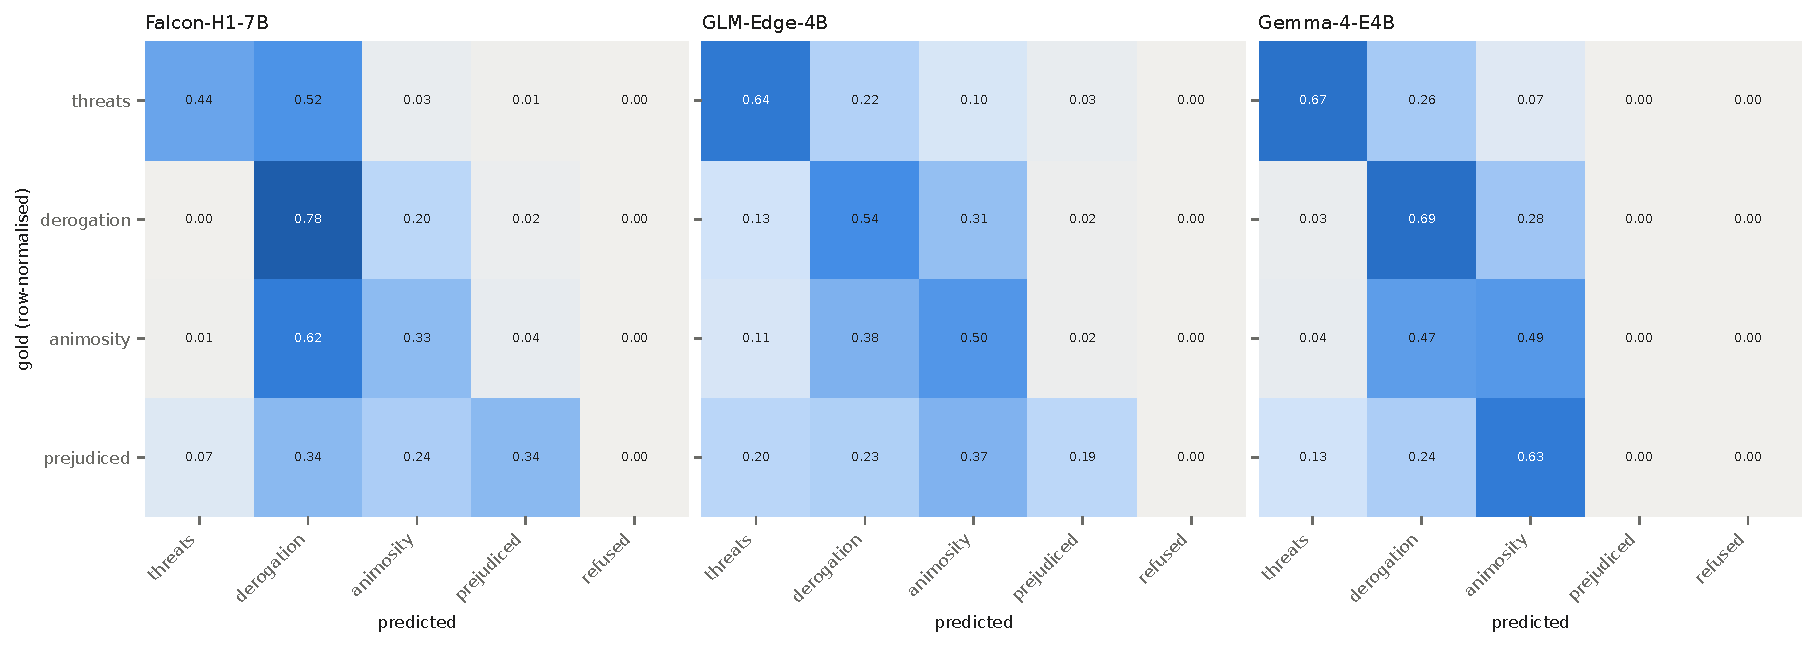
\includegraphics[width=\textwidth]{confusion_top3_task_b.pdf}
\caption{EDOS~B: row-normalised confusion matrices of the three best models on the 970 sexist test posts.}
\label{fig:confb}
\end{figure}

\begin{figure}[t]
\centering
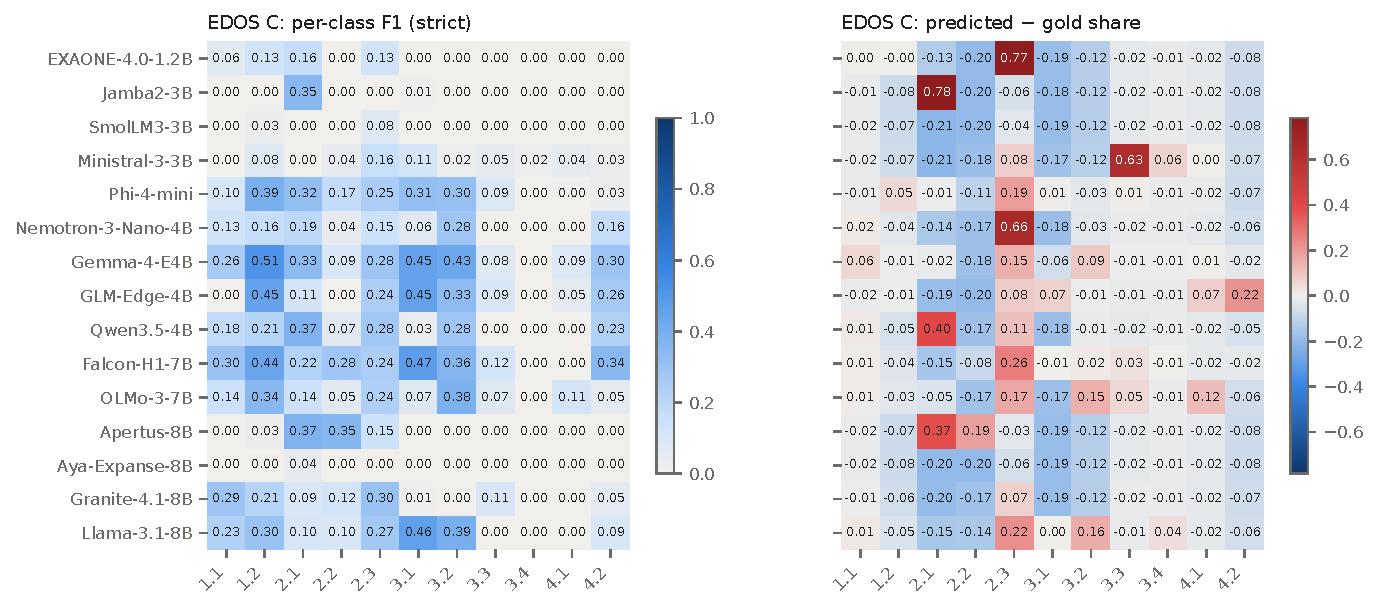
\includegraphics[width=\textwidth]{per_class_task_c.pdf}
\caption{EDOS~C: per-class F1 (left) and predicted minus gold class share (right; red: over-predicted).}
\label{fig:perc}
\end{figure}

\paragraph{EDOS~B.} The dominant confusion is between \emph{animosity} and \emph{derogation} (Figure~\ref{fig:confb}); Falcon-H1-7B labels 62\% of animosity posts as derogation. \emph{Prejudiced discussions} is the hardest category. Falcon-H1-7B recovers 34\% of these posts and GLM-Edge-4B 19\%, and 9 of the 15 models never predict this category. It is also the last option in the prompt. Because the option order was not permuted, a position effect cannot be separated from category difficulty.

\paragraph{EDOS~C.} Several models concentrate their predictions on a single vector (Figure~\ref{fig:perc}). Jamba2-3B assigns 2.1 (descriptive attacks) 78 percentage points more often than its gold share. EXAONE-4.0-1.2B and Nemotron-3-Nano-4B over-assign 2.3, and Ministral-3-3B over-assigns 3.3. This collapse explains their near-baseline macro-F1. The rarest vectors (3.3, 3.4 and 4.1) reach an F1 of at most 0.12 for every model.

\subsection{Over-prediction and calibration}
\tbl{calibration}

\paragraph{Positive rates.} With the a priori threshold of 0.5, models label more posts as sexist than the annotators do (Table~\ref{tab:calibration}). The gold rate is 0.321 on CMSB, where 14 of the 15 models predict a higher rate (up to 0.689). The gold rate is 0.242 on EDOS~A, where all 15 do (0.259--0.760).

\paragraph{Calibration.} The signed gap between the mean score and the gold rate is positive for the same 14 and 15 models. ECE ranges from 0.034 to 0.325 on CMSB and from 0.094 to 0.508 on EDOS~A. Among the posts that the three best EDOS~A models score above 0.9, 57\% (Gemma-4-E4B), 55\% (Jamba2-3B) and 75\% (SmolLM3-3B) are gold-sexist (Appendix Figure~\ref{fig:cal}). The raw scores should therefore not be read as probabilities.

\subsection{Agreement between models and model size}
\tbl{agreement}

\paragraph{Agreement.} Agreement among the 15 models is moderate on the binary tasks: Fleiss' $\kappa$ is 0.57 on CMSB, 0.43 on EDOS~A and 0.49 on EXIST~1.1, and it averages 0.44 over the five EXIST~1.3 labels. It is low on the multi-class tasks: 0.20 on EDOS~B, 0.12 on EXIST~1.2 and 0.05 on EDOS~C (Table~\ref{tab:agreement}).

\paragraph{Model size.} The Spearman correlation between model-card size and macro-F1 is 0.37 (CMSB), $-0.10$ (EDOS~A), 0.52 (EDOS~B; $p = 0.045$, uncorrected) and 0.27 (EDOS~C), as shown in Appendix Figure~\ref{fig:size}. With 15 models in a narrow range (1.28--8B), this indicates no consistent monotonic relation, but it cannot rule out a moderate size effect.

\subsection{EXIST 2025}\label{sec:exist}
The EXIST~2025 test gold labels are held by the organisers' evaluation platform, EvALL (\url{https://evall.uned.es}), which scores submitted predictions against them. We found no public release of these labels as of October 2026. EXIST~2025 is listed in the EvALL task repository, so predictions can be evaluated after the campaign.

For each model and task we prepared hard and soft submissions in the official format, in two variants:
\begin{itemize}
  \item non-answers left out of the submission;
  \item every tweet answered by arg-max ($\tau$ = none).
\end{itemize}
Coverage can therefore be reported alongside each score. Non-answers affect only Task~1.2, where Granite-4.1-8B, SmolLM3-3B and Ministral-3-3B leave out 164, 25 and 11 tweets. For Task~1.3 the soft value for ``not sexist'' is $\prod_{\ell}\bigl(1 - P(\text{Yes}_\ell)/m_\ell\bigr)$ over the five categories, which treats the categories as independent. The files pass the official format validator, apart from an instance-count check that assumes the full bilingual test set (2{,}076 tweets). The official measures (ICM, ICM-soft and F1) will be added once this evaluation is complete.

\section{Discussion}\label{sec:discussion}
\paragraph{Binary detection.} Without any training data, the best small models separate sexist from non-sexist posts with macro-F1 well above the majority baseline, and models of 3--4B parameters are among the best on both binary benchmarks. Performance varies strongly by dataset and by model, however. On EDOS~A the median model reaches only 0.577, and the best zero-shot score remains about 0.11 below the organisers' fine-tuned baseline. Zero-shot prompting therefore looks most useful as a starting point or for screening, rather than as a replacement for supervised detection.

\paragraph{Fine-grained categorisation.} Scores fall at each level of the EDOS hierarchy, and the errors are systematic rather than random. Neighbouring categories (animosity and derogation) are confused, rare vectors are almost never recovered, and several models fall back on a single vector. In our results this is where zero-shot models fall furthest short of supervised systems, and where task-specific training or richer definitions are most likely to help.

\paragraph{Answer format.} The same models that answer every Yes/No question can fail to produce a valid letter for most 11-way questions. Treating these cases as errors, or reading off the most likely letter regardless, changes some models' EDOS~C scores by up to 0.11 and changes their ranking. We therefore suggest that zero-shot evaluations on fine-grained label sets report non-answer rates next to their scores and state how non-answers were treated. The Gemma-4-E4B pattern also shows that a non-answer can carry information: most of its non-answers fall on posts to which no offered category applies.

\paragraph{Over-flagging.} With an uncalibrated threshold, almost every model predicts sexism more often than annotators do, and high scores overstate the probability that a post is sexist. In a moderation setting this would translate into many false flags. Calibrating the decision threshold on labelled development data is the natural next step; we did not test it in this study.

\section{Conclusion}\label{sec:conclusion}
Small open language models used zero-shot detect sexism well above chance on two binary benchmarks, but they remain far from supervised performance on fine-grained categorisation. Their measured performance on multi-class tasks depends substantially on whether they answer in the required format. Evaluations of such models should report non-answers per label, fix their scoring rules in advance, and compare models with paired tests rather than point estimates. The supervised models trained on the reserved training and development data, and the official EXIST evaluation, will complete this comparison.

\section{Limitations}\label{sec:limits}
\paragraph{Decision rules.} The decision threshold and the non-answer threshold were fixed a priori, so no labelled data influenced the scores. The thresholds are not calibrated, and calibrated thresholds would likely change the binary results and possibly the ranking (Section~\ref{sec:discussion}).

\paragraph{Prompt and scoring choices.} Each task uses a single prompt with a fixed option order and abridged category definitions. Prompt wording and formatting are known to affect results \citep{reuver2025tell,sclar2024quantifying}, and the option order may favour some classes (Section~\ref{sec:results}). Labels are read from the first reply token, which can differ from the answer a model would write out \citep{wang2024myanswer}. A non-answer conflates format non-compliance with declining to answer. Reasoning modes were disabled, because first-token scoring is incompatible with them.

\paragraph{Coverage.} The study covers open models of up to 8B parameters and English data only. Because EDOS and CMSB were public before these models were trained, their test texts may appear in pre-training data. The CMSB split is our own, and the EXIST scores are pending the official evaluation.

\section*{Ethics statement}
This work uses three public research datasets under their terms of use and involves no new annotation. No example posts are reproduced. Sexism annotation is subjective, and gold labels reflect the annotators' judgements. EXIST preserves annotator disagreement explicitly. Automated sexism classifiers can harm users when deployed without care. The over-prediction found here would lead to many false flags, and reported or critical speech about sexism (EXIST~1.2 intentions) can be mistaken for sexism itself. We do not recommend deploying the evaluated models for content moderation without calibration, human review and evaluation on the target platform. Two of the models carry non-commercial licences (Appendix Table~\ref{tab:models}).

\section*{Code and data availability}
The evaluation code, prompts, the CMSB split, the per-post predictions with their full answer-token distributions, and the EXIST submission files will be made available with the paper. Each of the 105 model--task evaluations records its configuration, pinned model revision, software versions and hardware. An automated audit confirmed that every evaluation is complete, contains no duplicate posts, used the pinned revision and used a single prompt version.

\bibliographystyle{plainnat}
\bibliography{refs}

\clearpage
\appendix
\section{Models}\label{app:models}
\tbl{models}
\FloatBarrier

\section{Implementation details}\label{app:impl}
All evaluations used PyTorch 2.11.0 (CUDA 13.0) and Transformers 5.20.1 on an NVIDIA A100-SXM4-80GB. Two models (Aya-Expanse-8B and Jamba2-3B) were evaluated from a later code revision whose inference and scoring code is identical to that of the other 13 models. A single label score lies exactly at the decision threshold (one EXIST~1.3 label of Gemma-4-E4B); it is predicted positive under the $\geq 0.5$ rule.

\section{Prompts}\label{app:prompts}
The exact system and user messages, with a placeholder in place of the post. Each was formatted with the model's chat template.

\small
\tbl{prompts}
\normalsize
\FloatBarrier
\clearpage

\section{Additional results}\label{app:results}
\tbl{significance}
\tbl{secondary}
\tbl{sensitivity}

\begin{figure}[!htbp]
\centering
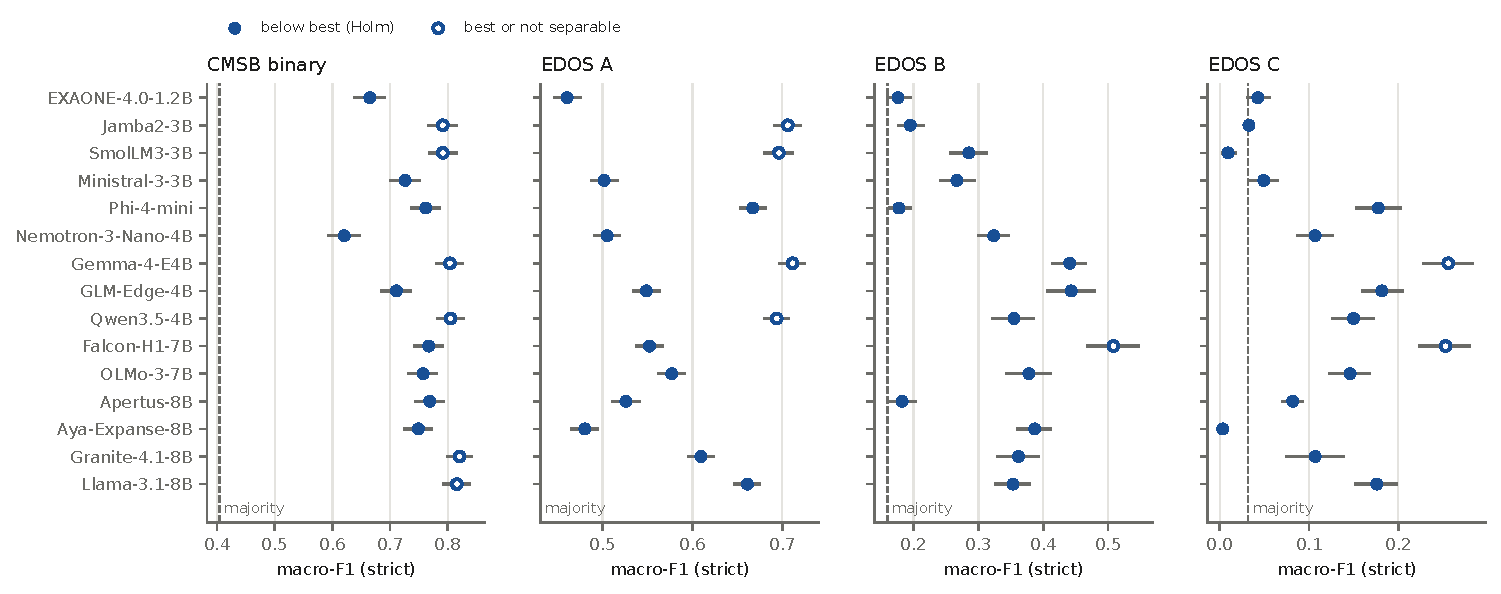
\includegraphics[width=\textwidth]{main_macro_f1_ci.pdf}
\caption{Test macro-F1 with 95\% bootstrap confidence intervals ($\tau = 0.5$). Models are ordered by size. Hollow markers: the best model and models not significantly different from it; dashed line: majority-class reference.}
\label{fig:main}
\end{figure}

\begin{figure}[!htbp]
\centering
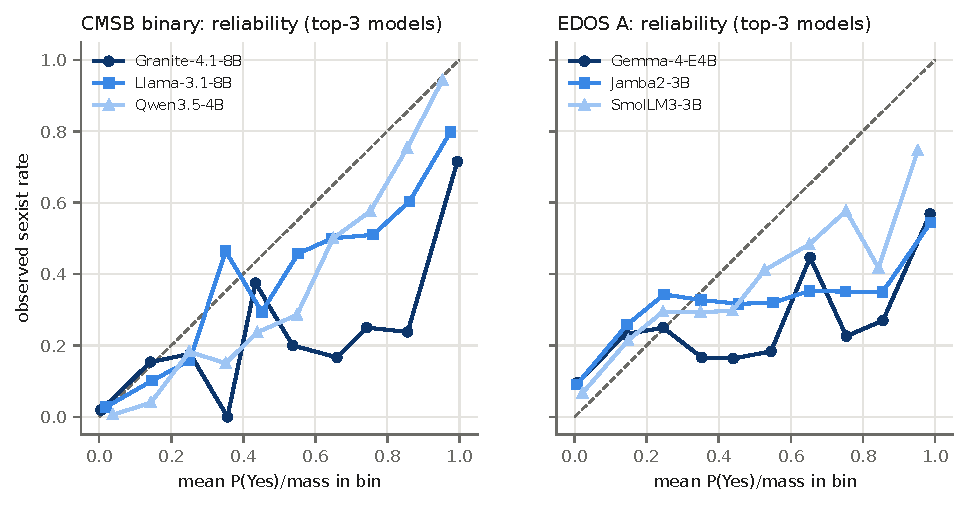
\includegraphics[width=0.8\textwidth]{calibration_top3.pdf}
\caption{Reliability diagrams of $P(\text{Yes})/m$ for the three best models on each binary task (10 equal-width bins).}
\label{fig:cal}
\end{figure}

\begin{figure}[!htbp]
\centering
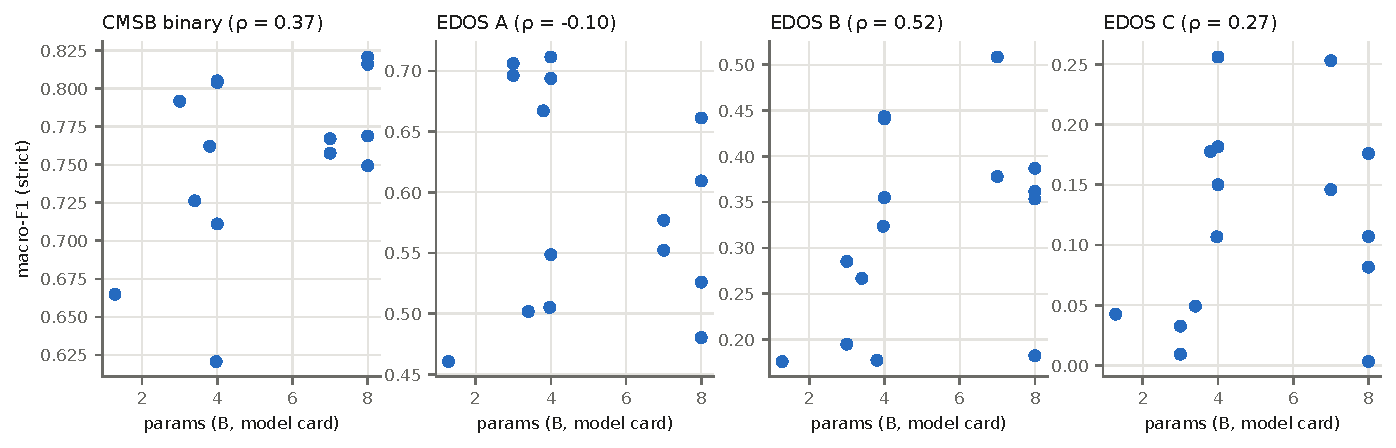
\includegraphics[width=\textwidth]{size_vs_f1.pdf}
\caption{Model-card parameter count against test macro-F1 (Gemma-4-E4B is plotted at its effective size of 4B).}
\label{fig:size}
\end{figure}

\begin{figure}[!htbp]
\centering
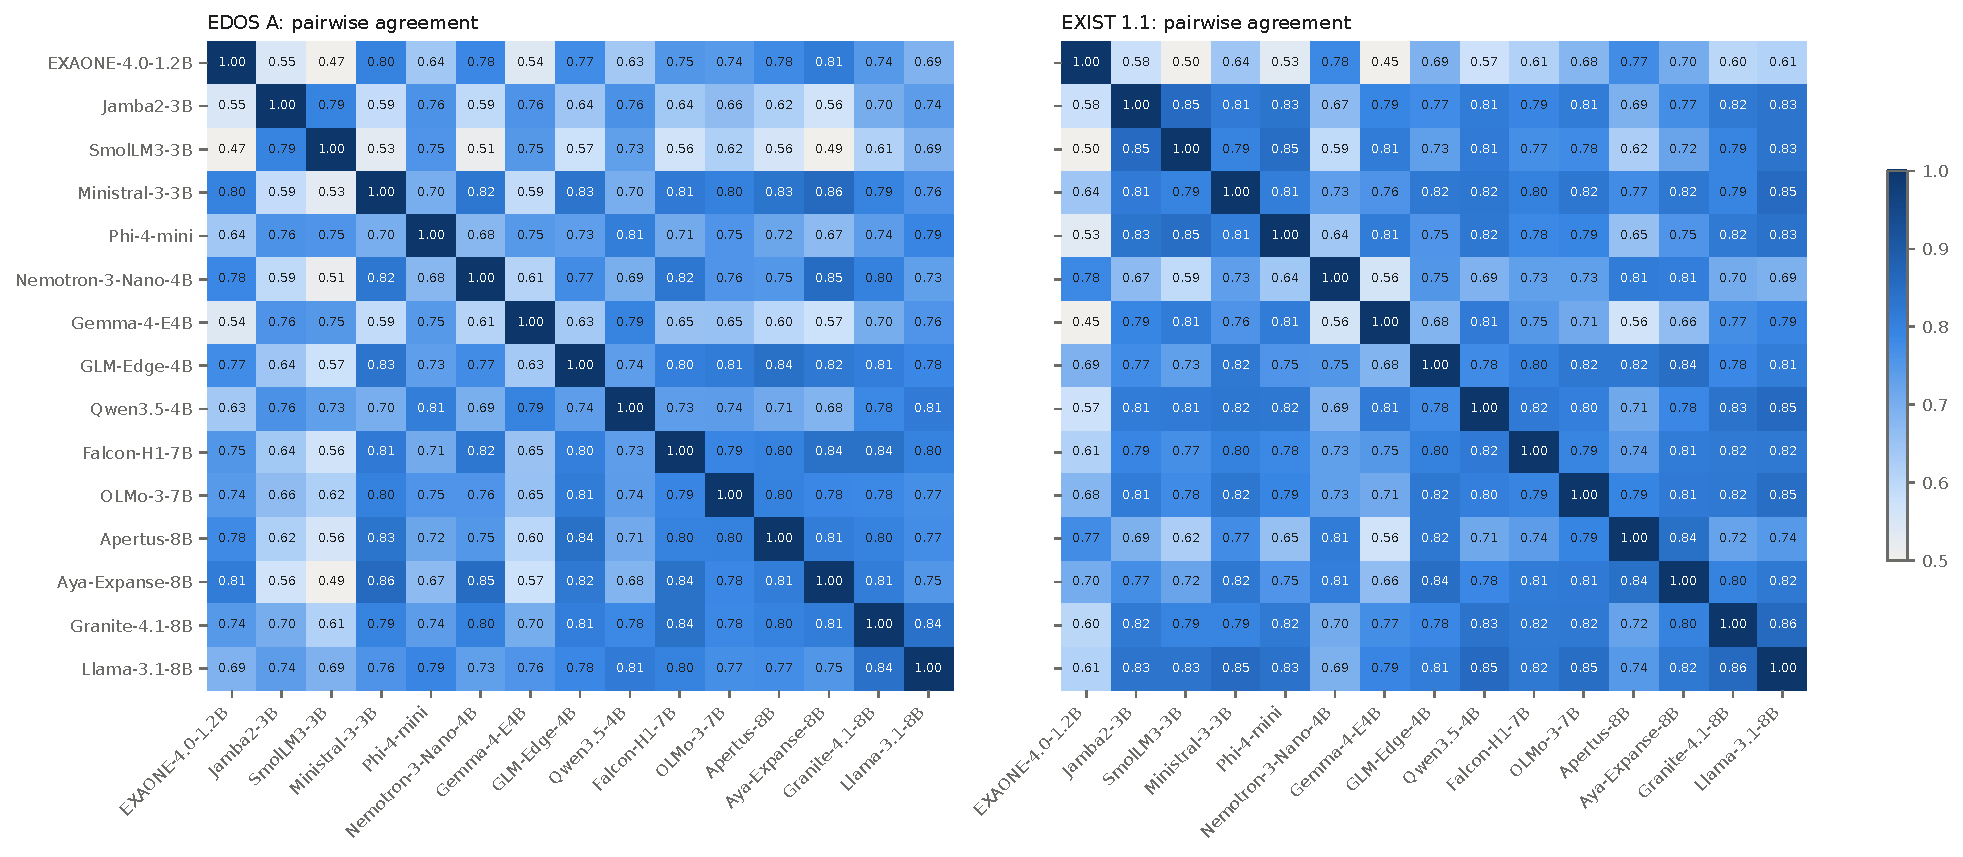
\includegraphics[width=\textwidth]{pairwise_agreement.pdf}
\caption{Share of test posts on which two models give the same prediction (a non-answer counts as its own prediction).}
\label{fig:pair}
\end{figure}

\end{document}
